

\frame{\frametitle{Operations more than  development}
   \begin{itemize}
	\item  Agile works well for development - there is a product to be built
	\item  Operations uses that product, finds bugs which need fixing, needs enhancements
	\item  Development does not disappear but does tend more to maintenance
	\item  Configuration control is even more important...
	\item  Operations are more procedural, a little more repetitive (we hope), routine (we really hope)
	\item It is a different mindset - a stable running system is the prime objective  
	
   \end{itemize}
}


\frame{\frametitle{ Operations rehearsals}
\begin{itemize}
\item We choose to have operations rehearsals for Gaia - {\color{red} These are not software test campaigns } we had those as well.
\item OR\#1:
	\begin{itemize}
	\item 3 days of NSL data
	\item DPCE (SCI) operations
	\item Other DPCs data reception only
	\end{itemize}

\item OR\#2:
	\begin{itemize}
	\item 5 days of EPSL data (less volume over time)
	\item All DPCs operational - almost all daily chains
	\item Commissioning activities (payload experts introduced)
	\end{itemize}
\item OR\#3:
	\begin{itemize}
	\item 8 days of EPSL data
	\item All DPCs operational - all daily chains
	\item Commissioning activities (payload experts continued)
	\end{itemize}
\end{itemize}
}


\frame{\frametitle{It is not easy .. some comment }
\begin{itemize}
\item on OR\#1
	\begin{itemize}
	\item “Mindset has to change from development to operations”
	\end{itemize}
\item  after OR\#2
	\begin{itemize}
	\item “Again, the SCIs came late; too late to allow DPCE to conduct any substantial testing and integration. This would lead to the same consequences as seen already during OR\#1”
	\item In plain words: completely unknown SW behaviour, limited to no robustness of systems to unexpected events and data, processing break-down after about 30hours of data

	\end{itemize}
\item UB statement after OR\#2
	\begin{itemize}
	\item “The design of the OR was not adequately set and many details were missing.” 
	\end{itemize}

\end{itemize}
}

\frame{\frametitle{ Operations Rehearsal:Group interactions} 
\begin{center}
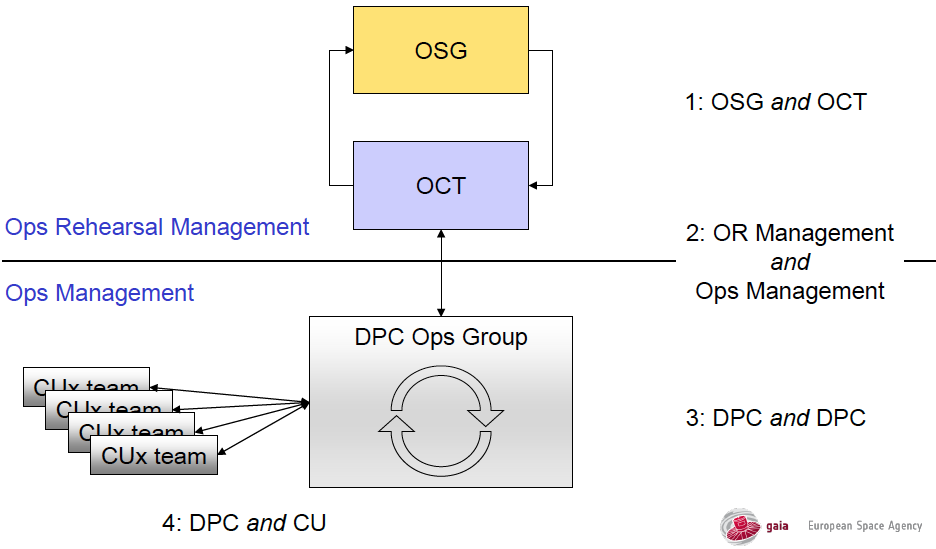
\includegraphics[width=\textwidth]{images/gaiaORgroups}
\end{center}
{\tiny \bf Sebastian Els }
}

\frame{\frametitle{Payload Experts - is there an LSST equivalent ? }
\begin{itemize}
\item Basic roster on second OR ..  Daily ~1h telecons to exchange on findings
	\begin{itemize}
	\item Started well, but seemed to cool down after about a week
	\item Use of Mantis to track issues and to raise them to MOC/Project/Astrium
	\item Some work seems to be hidden in FL reports; unawareness of where to find raw FL results
	\end{itemize}
\item Operational awareness of PEs  improved
\item Finally, also HK data (other than attitude) were looked at
\item The responsibility of the PEs for on-board changes was exercised
	\begin{itemize}
	\item a bit ad-hoc, but still the need for CC seems accepted (at least by most)
	\item CCB process executed for VO sequence and ALPT (the change of compression parameters was not part of this exercise)
\item Needs for improvement
	\begin{itemize}
	\item Definition of the process of how to request final approval
	\item Detailed process during commissioning (Astrium is in charge)
	\end{itemize}
	\end{itemize}
\end{itemize}
}


\frame{\frametitle{ Procedures .. post ops rehearsal}
\begin{itemize}
\item “Procedures are the building blocks for operations” 
\begin{itemize}
\item 118 procedures in DPCE Procedure Handbook + CSG – Gaia Ops Procedure
\item Half of them were used in OR4. Many of them were out of date or
not validated. Some new ones have been identified
\item We operators must be trained and educated on their regular use
\end{itemize}
\item Procedure Handbook in pdf is not very friendly for operators
\item Proposal to move the handbook to entries in eLog – more
handy and friendly. Can be tracked and controlled in the
same way (Currently like that - others looking at JIRA/Confluence)
\item logging more of a problem 
\end{itemize}
{\tiny \bf Rocio Guerra Ops Manager Gaia ESAC}
}

\frame{\frametitle{Regular Operations Exercises (ROEs) }
\begin{itemize}
\item Operations rehearsals took a lot of time tom plan - so they were not more than once a year.
\item It is not acceptable to have system diverge in this time period
\item  Need a continuous (super)integration – at least on a monthly basis -
\item Done with the trunks
\item Need  a plan including
\begin{itemize}
\item Schedule – basically to reserve time for this
\item Objectives - can be to improve on finding from one of the operations rehearsals
\item Input dataset - can reuse again from ops rehearsal or reduced version
\end{itemize}
\end{itemize}
}


\frame{\frametitle{ Who does operations ?}
\begin{itemize}
\item Who is the science operations manager ?
\item Who are the operations people ?
\end{itemize}
}



\frame{\frametitle{ }
\begin{itemize}
\item \ldots
\end{itemize}
}




